\documentclass[A4]{scrartcl}
\usepackage[paper=a4paper,left=10mm,right=10mm,top=25mm,bottom=25mm]{geometry}
\usepackage[utf8]{inputenc}
\usepackage{graphicx}

%SS2017P komplett
%SS2017 komplett

\begin{document}
  \addsec{Verständnisfragen}
  Welche zwei Parameter bestimmen die Bandbreite einer rückgekoppelten\\ 
  Operationsverstärkerschaltung?\\
  \bigskip Antwort: Bandbreite des OP (Transitfrequenz) $F_t$ + Verstärkung der Rückkopplung ($A_0$)\\
  Welche zwei Eigenschaften sind für einen VC-operationsverstärker charakteristisch?\\
  \bigskip Antwort: Eingangswiderstand ist sehr groß (Spannungseingang), Ausgangswiderstand ist sehr groß(Stromausgang)\\
  Im Handel sind verschiedene Arten von Operationsverstärkern verfügbar. Diese werden durch zwei Buchstaben beschrieben: XY-Operationsverstärker. 
  Was wird durch die Buchstaben beschreiben und welche Optionen sind verfügbar?\\
  Antwort: X = Eingang, Y = Ausgang\\
  V = Spannungs-Ein/Ausgang, C= Strom-Ein/Ausgang.\\
  \bigskip Verfügbar sind: VV,VC,CV,CC - Operationsverstärker \\
  Worauf müssen sie bei der Verwendung eines VC-Operationsverstärkers achten?\\ 
  Erklären sie am Beispiel eines Spannungsfolgers.\\  
  \bigskip Antwort: Bei der Rückführung muss der Ausgangsstrom in eine Spannung konvertiert werden (z.B. über einen Widerstand), deshalb ist eine direkte Verbindung von Ausgang und Eingang nicht Möglich.\\
  Was bzw. welches Bauteil definiert die Eingangsimpedanz einer nicht-invertierenden Verstärkerschaltung?\\
  \bigskip   Antwort:Der Eingangswiderstand des OP's\\
  Was versteht man unter der common mode rejection ratio CMRR?\\  
  Antwort: Die Fähigkeit eines realen Operationsverstärkers seinen Ausgang bei Symmetrischen Eingangssignalen möglichst wenig zu ändern.\\
  (Symmetrische Änderungen des Eingangs haben aufgrund von Assymetrien/Nichtidealitäten an den Eingängen eine Änderung am Ausgang zur Folge)\\
  \bigskip Sie ist damit ein Maß für den Einfluss der Eingangsspannung auf die Ausgangsspannung.\\
  CMRR = Common Mode Rejection Ratio\\
  Was versteht man unter power supply rejection Ratio PSRR?\\
  \bigskip Antwort: Die PSRR gibt ein Maß für den Einfluss der Versorgungsspannung auf den Ausgang an.\\
  Erläutern Sie die Unterschiede zwischen einem normalen Operationsverstärker, einem single Supply und einem rail-to-rail OP? (Eventuell fertigen Sie zur Erklärung eine kleine Skizze an).\\
  Antwort: \\
  normaler OPV (Symmetrische Versorgung): Versorgung mit $+U_V$, $-U_V$, Nutzbereich $\approx [(-U_V +1/2V); (+U_V -1/2)V]$\\
  single Supply OPV (Asymmetrische Versorgung): Versorung mit $+U_V$, Nutzbereich $\approx [(0V+ "x"mV); (Uv -1/2V)]$ \\
  \bigskip Rail to Rail OPV (Symmetrische Versorgung): Versorung mit $+U_V$, $-U_V$, Nutzbereich $\approx [(-U_V + "x"mV); (+U_V - "x"mV)]$\\
  Nennen sie zwei OP-Grundschaltungen, die häufig für die Realisierung von Filtern höherer Ordnung verwendet werden.\\
  \bigskip 
  Antwort: Sallen - Key Filter, Multiple Feedback Filter, Universal/State-Variable-Filter\\
  Warum können Sie einen Operationsverstärker als Komparator einsetzen, einen Komparator aber nicht als Operationsverstärker?\\
  \bigskip 
  Antwort: Der Ausgang des Komparator kann meist nur $+U_s$ und $-U_s$\\
  \newpage
  Was sind die charakteristischen Eigenschaften eines Instrumentenverstärkers?\\
  Antwort: sehr hoher Eingangswiderstand, dadurch wenig Beeinflussung der Messung durch Nichtidealitäten.\\
  Wann wird er verwendet?\\
  \bigskip 
  Antwort: Präzise Messschaltungen und Messung\\ von Schaltungen mit hohen Ausgangswiderständen.\\
  Skizzieren sie das Blockschaltbild für einen (Einquadranten-)Analogmultiplizierer? Aus welchen Grundelementen wird dieser typischerweise aufgebaut?\\
  \bigskip 
  Antwort:\\
  Wozu dient die Frequenzgankompensation in einem Operationsverstärker? Nennen sie zwei typische Implementierungen.\\
  \bigskip Antwort:??? \\ 
  Erklären sie, warum bei einem vereinfachten Dreiecksgenerator nicht immer ein Dreieck am Ausgang entsteht? Von welchen Bauteilen ist dies abhängig(Skizze)?\\
  \bigskip Antwort: ???\\
  Was bzw. welches Bauteil definiert die Eingangsimpedanz einer invertierenden Verstärkerschaltung?\\
  \bigskip Antwort: ???\\
  Was bzw. welches Bauteil definiert die Eingangsimpedanz einer Integratorschaltung?\\
  \bigskip Antwort: Der Widerstand vor dem Kondensator.\\
  Warum setzt man in der Praxis eine reine Integratorschaltung nur selten ein? Unter welchen Bedingungen/in welchen Schaltungen wird sie dennoch verwendet? 
  Warum ist die Verwendung dort möglich?\\
  Antwort: Die reine Integratorschaltung stellt einen Tiefpass dar und ist nur bei Frequenzen $F >> f_C$\\
  ein Integrierer(Linearität der E-Fkt der Ladekurve)\\
  Da die Nichtidealitäten (Offset- und Basisströme) mit integriert werden, neigt der Integrierer dazu sich über die Laufzeit auf einer der Versorgungsspannungen festzulegen.\\
  Ein Integrierer ist bei niedrigen Frequenzen deshalb nur mit einem Parallelwiderstand\\
  \bigskip oder einer automatischen Entladeschaltung nutzbar.\\
  Nennen sie zwei Optionen um das Weglaufen der Ausgangsspannung in einer Integratorschaltung zu verhindern? Wann verwenden sie welche Option ?\\
  \bigskip Antwort: Entladewiderstand parallel zum Kondensator , Entladeschaltung (vgl. Öffner)\\
  Nennen Sie drei in der Vorlestung diskutierte Filtercharakteristiken.\\
  \bigskip Antwort: Bessel, Butterworth, Tschebyscheff, Kritische Verstärkung, Cauer-Filter.\\
  Erläutern sie den Unterschied zwischen der Eigenfrequenz $f_0$ und der Grenzfrequenz $f_c$ eines Tiefpasses 2. Ordnung.\\
  Antwort:\\
  $f_c = $ Frequenz bei der der Ausgang Verstärkung-3DB beträgt (Bsp: $A_0 = 10dB - 3dB = 7dB $)\\
  \bigskip $f_0 = $ Frequenz bei der$\varphi(f_0) = -90^\circ$\\
  Ein state-variable-Filter wird häufig als Universal-Filter bezeichnet. Erklären Sie warum?\\
  Antwort: 1. man kann mit einem State Variable Filter alle Filtertypen (gleichzeitig) realisieren\\
  \bigskip (Hochpass, Tiefpass, Bandpass, Bandsperre).
  \newpage
  Sie möchten einen invertierenden Verstärker bauen. in Ihrer Bastelkiste finden sie aber nur einen LM339 Komparator IC. Was machen sie? Warum?\\
  Antwort: IC ist nicht nutzbar, da Ausgang nur Totem-Pole-Endstufe($ +U_S$, $-U_S$)\\
  \bigskip Keine Zwischenwerte möglich, daher: neue IC's bestellen (man kann einenen Komparator nicht als OPV nutzen)\\
  Warum werden die Eigenschaften der meisten Operationsverstärkerschaltungen nicht durch die Eigenschaften des Operationsverstärkers, sondern im Wesentlichen durch die externen Komponenten bestimmt ?\\
  \bigskip Antwort: $\frac{U_out}{U_in} = \frac{G}{1-G\cdot H} = -\frac{1}{H}$ für $G\cdot H >> 1$\\
  Sie haben im Labor eine ideale Differenzierer-Schaltung aufgebaut.\\
  Zum Testen der Schaltung verwenden sie ein Dreieckssignal.\\
  Leider hat das Ausgangssignal keinen rechteckförmigen Verlauf, sondern seltsame "Zacken" an den Flanken.\\
  Sie haben festgestellt das die "Zacken" mittels eines Widerstands in Reihe zum Kondensator entfernen können.\\
  Erklären sie wodurch die "Zacken" entstehen und warum sie mit dem Widerstand entfernt werden können. Eventuell hilft eine Zeichnung weiter.\\
  Antwort: Der Operationsverstärker wird durch den Kondensator kapazitiv belastet.\\
  Dies verursacht Stabilitätsprobleme (System 2. Ordnung) der Kondensatorladestrom,\\
  \bigskip wird durch den Widerstand begrenzt.\\
  Was versteht man unter der Phasenreserve eines rückgekoppelten Systems?\\
  Antwort: Phasenreserve $ \varphi_r = 180^\circ - \varphi$\\
  Bei einer Verstärkung von $|A|=0dB=1$\\
  \bigskip Maß für die Stabilitätsreserven eines Systems\\
  Erklären sie Stichpunktartig den Unterschied zwischen Differenzverstärker und einem Differenzierer?\\
  Antwort:
  Differenzverstärker: Verstärkt die Differenz zwischen invertierenden und nicht invertierenden Eingang (Math. Operation der Subtraktion)\\
  \bigskip Differenzierer: Führt die Operation der Differentiation auf ein Eingangsfunktional aus.\\
  Warum können Sie in einem Rechteck-Dreieck Generator einen idealen integrator einsetzen und benötigen keinen Tiefpass?\\
  Antwort: Der Integrator wird kontinuierlich Ge-und Entladen,\\
  \bigskip er wird deswegen in einer Art Rückkopplung betrieben.\\
  Nennen Sie drei Filtertypen, die häufig für die Auslegung von Filtern höherer Ordnung verwendet werden.\\
  \bigskip Antwort: Bessel, Butterworth, Tschebyscheff, Kritische Dämpfung\\

  \addsec {OPV-Schaltungen}

  Gegeben sei folgende Schaltung:\\
  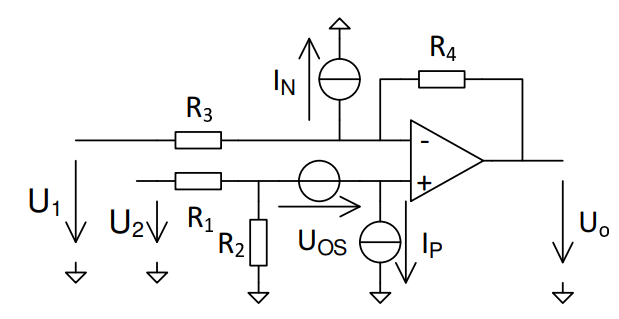
\includegraphics{Schaltung1.png}\\
  a) Bestimmen Sie die Ausgangsspannung $U_{out}$ als Funktion der gegebenen Größen.\\
  $U_{out} = f(U_1,U_2,U_{os},I_N,I_P)$\\
  b) Vereinfachen sie den Ausdruck für $R_1 = R_3, R_2 = R_4$ und $I_N = I_B + 0.5 I_{OS}, I_P = I_B-0,5I_{OS}$\\\\

  Gegeben sei folgende Schaltung:\\
  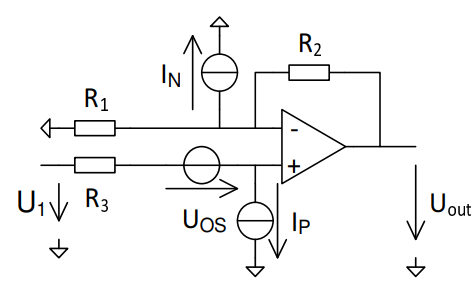
\includegraphics{Schaltung8.png}\\
  a) Bestimmen Sie die Ausgangsspannung $U_{out}$ als Funktion der gegebenen Größen.\\
  $U_{out} = f(U_1,U_{OS},I_N,I_P)$\\
  b) Vereinfachen sie den Ausdruck mittels $I_N = I_B + 0.5 I_{OS}, I_P = I_B-0,5 I_{OS}$.\\
  Dimensionieren sie $R_3$ so , dass der Einfluss des Eingangsruhestroms auf die Ausgangsspannung minimiert wird.\\\\

  Die Aussteuergrenzen sollen mit $\pm 15V$ angenommen werden.\\
  a) Schreiben sie jeweils die Potentiale bzw. Ströme in die Kästchen:\\
  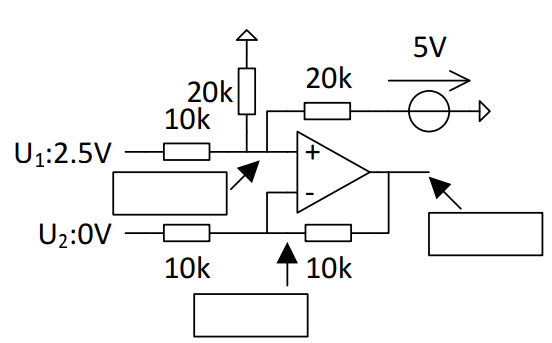
\includegraphics{Schaltung2.png}\\\\
  b) Schreiben sie jeweils die Potentiale bzw. Ströme in die Kästchen:\\
  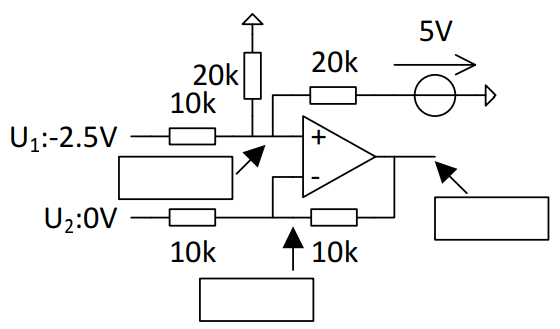
\includegraphics{Schaltung3.png}\\\\
  c) Schreiben sie jeweils die Potentiale bzw. Ströme in die Kästchen:\\
  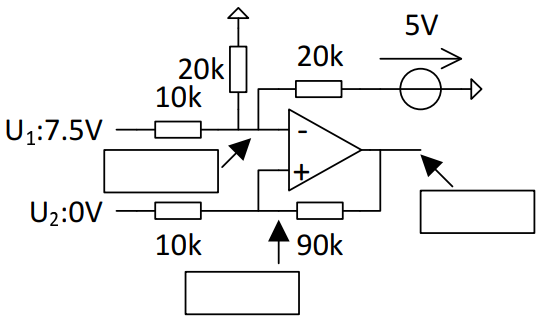
\includegraphics{Schaltung4.png}\\\\
  d) Schreiben sie jeweils die Potentiale bzw. Ströme in die Kästchen:\\
  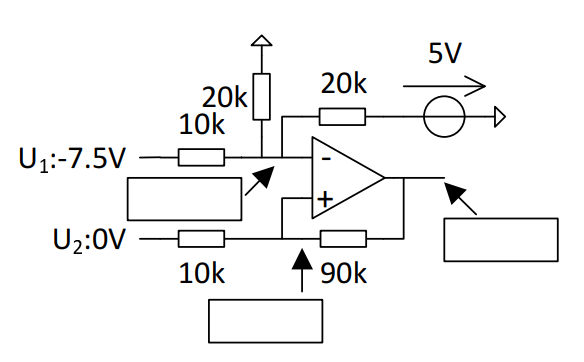
\includegraphics{Schaltung5.png}\\\\
  e) Schreiben sie jeweils die Potentiale bzw. Ströme in die Kästchen:\\
  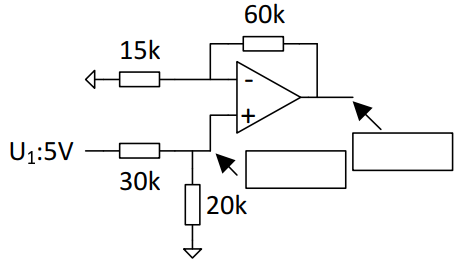
\includegraphics{Schaltung9.png}\\\\
  e) Schreiben sie jeweils die Potentiale bzw. Ströme in die Kästchen:\\
  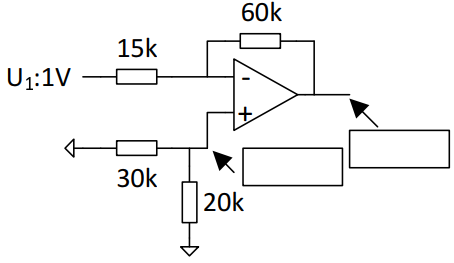
\includegraphics{Schaltung10.png}\\\\
  f) Schreiben sie jeweils die Potentiale bzw. Ströme in die Kästchen:\\
  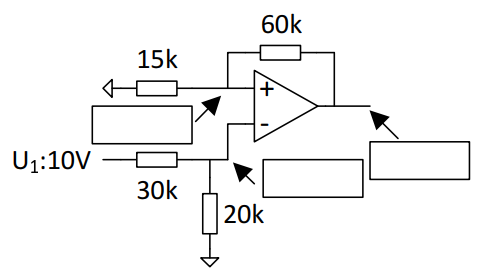
\includegraphics{Schaltung11.png}\\\\
  g) Schreiben sie jeweils die Potentiale bzw. Ströme in die Kästchen:\\
  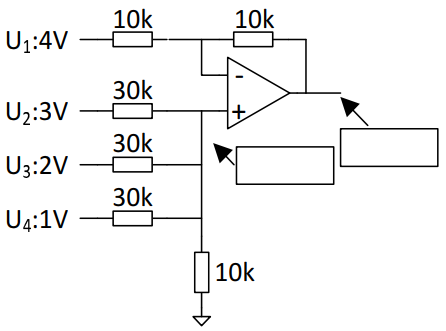
\includegraphics{Schaltung12.png}\\\\
  h) Schreiben sie jeweils die Potentiale bzw. Ströme in die Kästchen:\\
  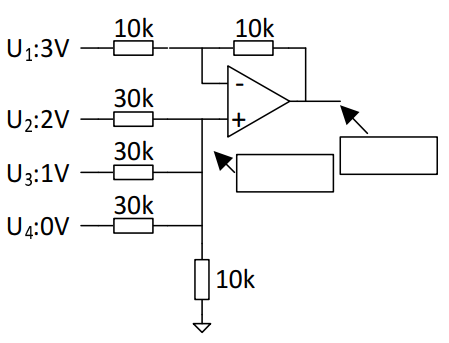
\includegraphics{Schaltung13.png}\\\\

  Gegeben sei folgende Schaltung:\\
  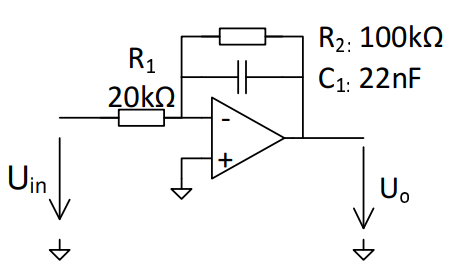
\includegraphics{Schaltung6.png}\\
  a) Um welche Grundschaltung handelt es sich ?\\
  b) Leiten Sie die Laplace-Übertragungsfunktion der Schaltung her.\\\\
  Skizzieren Sie im Folgenden den Verlauf der Augangspannung für eine rechteckförmige Eingangsspannung der Amplitude $\pm 1V$, ein Tastverhältnis von $50\%$ und verschiedene Frequenzen.
  Berechnen sie die Amplitude/Maximalwerte der Ausgangsspannung.\\
  Annahme: Die Signale liegen bereits seit langer Zeit an.\\
  c)Eingangssignal: $f=1Hz$\\
  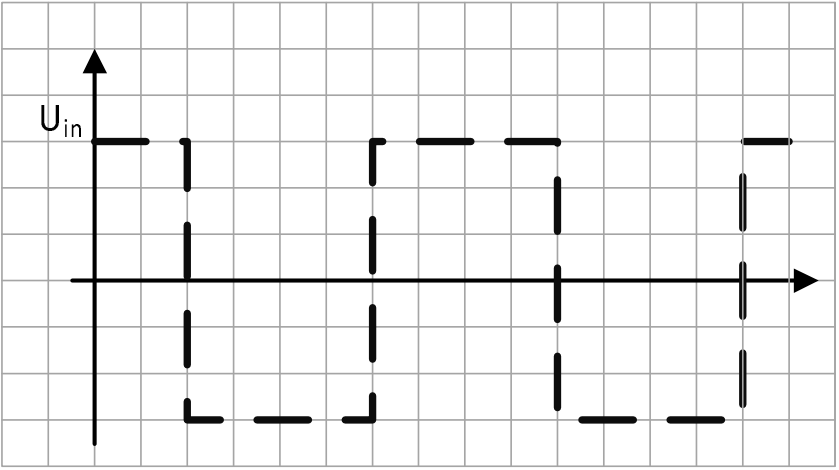
\includegraphics{U_rechteck.png}\\
  d)Eingangssignal: $f=100Hz$\\
  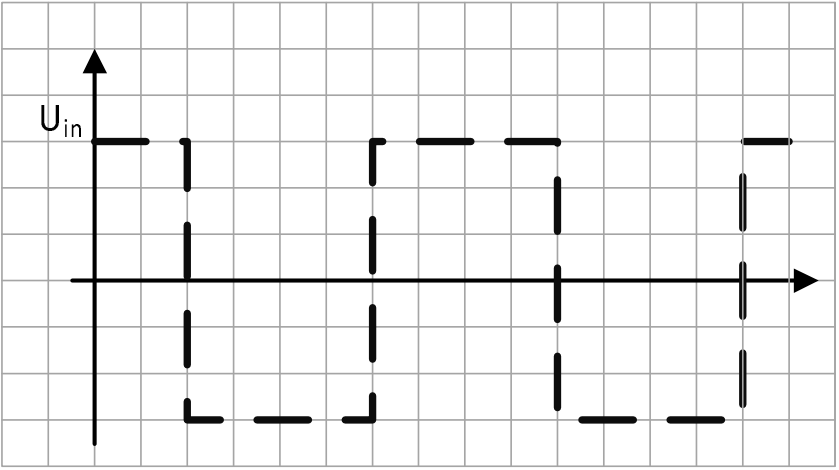
\includegraphics{U_rechteck.png}\\
  e)Eingangssignal: $f=1kHz$\\
  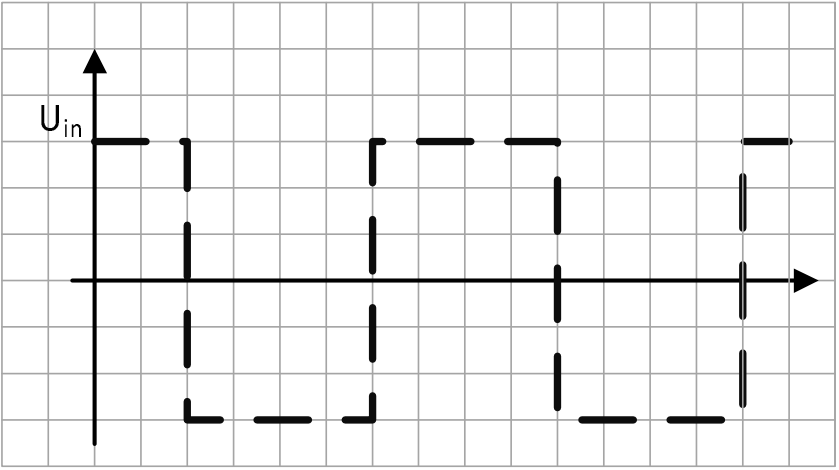
\includegraphics{U_rechteck.png}\\
  Gegeben sei folgende Schaltung:\\
  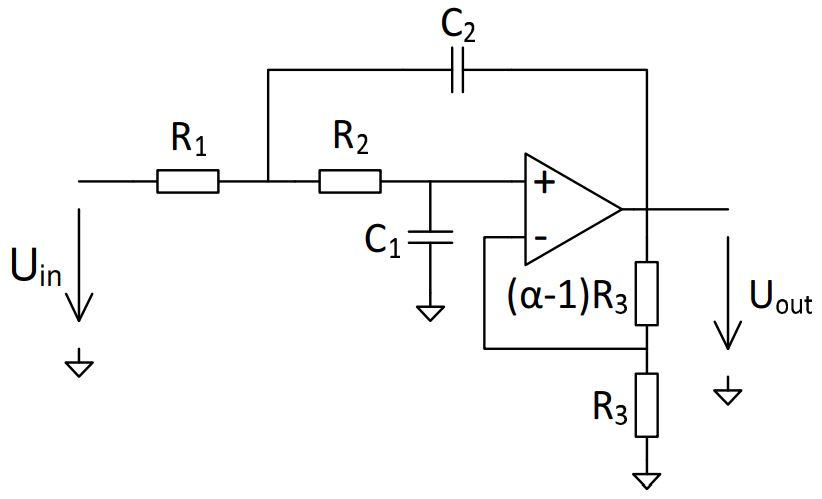
\includegraphics{Schaltung7.png}\\
  Die Übertragungsfunktion lautet: $G(s) = \frac{U_{out}(s)}{U_{in}(s)} = \frac{\alpha}{R_1R_2C_1C_2s^2+((R_1+R_2)C_1+(1-\alpha)R_1C_2)s+1}$
  a) Um welche Filterschaltung handelt es sich ?\\
  b) Vereinfach Sie die Übertragungsfunktion unter der Annahme , dass die Kondensatoren identisch sind ($C=C_1=C_2$) und die Widerstände in einem festen Verhältnis m stehen ($R_1=mR, R2=R$)\\
  c) Vereinfach Sie die Übertragungsfunktion unter der Annahme , dass die Kondensatoren und Widerstände jeweils identisch sind ($C=C_1=C_2 R=R_1=R_2$)\\
  d) Bestimmen sie durch Koeffizientenvergleich die Verstärkung $A_0$, die Eigenfrequenz $f_0$ und die Güte $Q$ des Systems.\\
  e) Bestimmen sie die Bauteilwerte $C$,$R_1$,$R_2$ für ein Filter mit folgenden Eigenschaften:\\
  $A_0 = 2,f_0 = 100kHz, Q=0,707$.\\
  f) Bestimmen Sie die Bauteilwerte $C,R$ sowie $\alpha$ für ein Filter mit folgenden Eigenschaften: 
  $f_0 = 100kHz, Q=0,5$
  Verwenden Sie Kondensatoren aus der E12 und Widerstände aus der E24 Reihe.\\
  g) Skizzieren sie den Amplitudengang und die Sprungantwort des Filters aus e).\\
  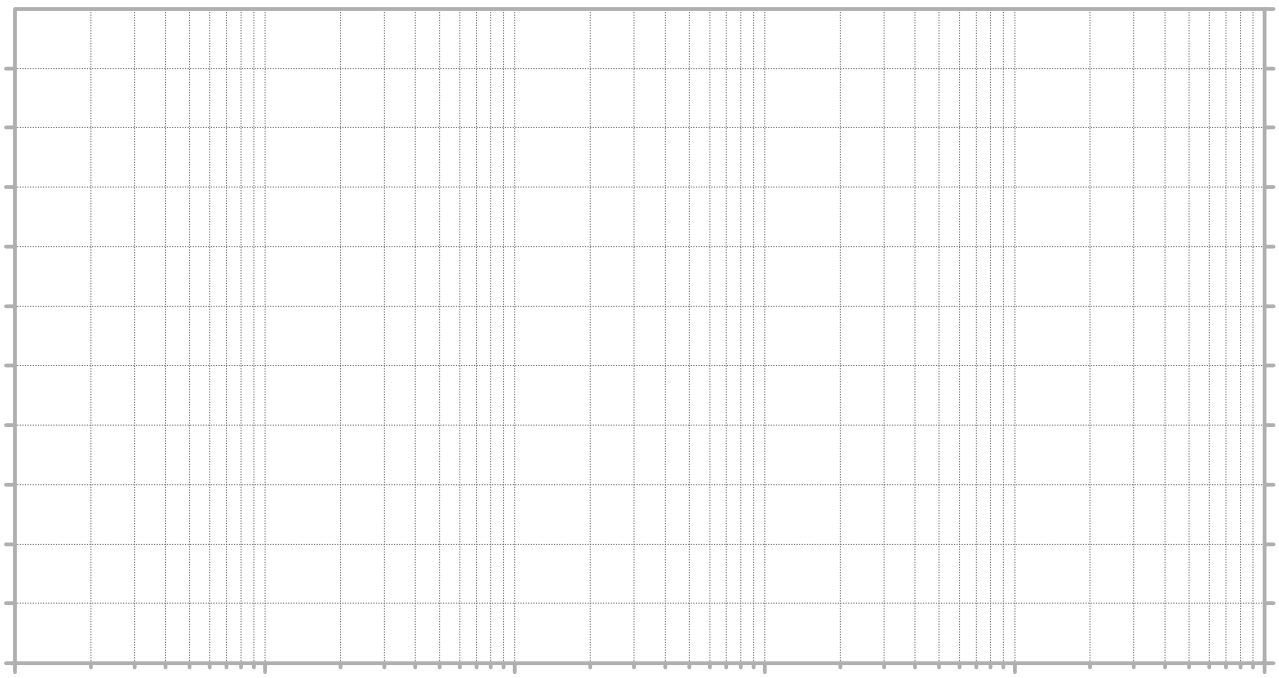
\includegraphics{logpaper.png}\\
  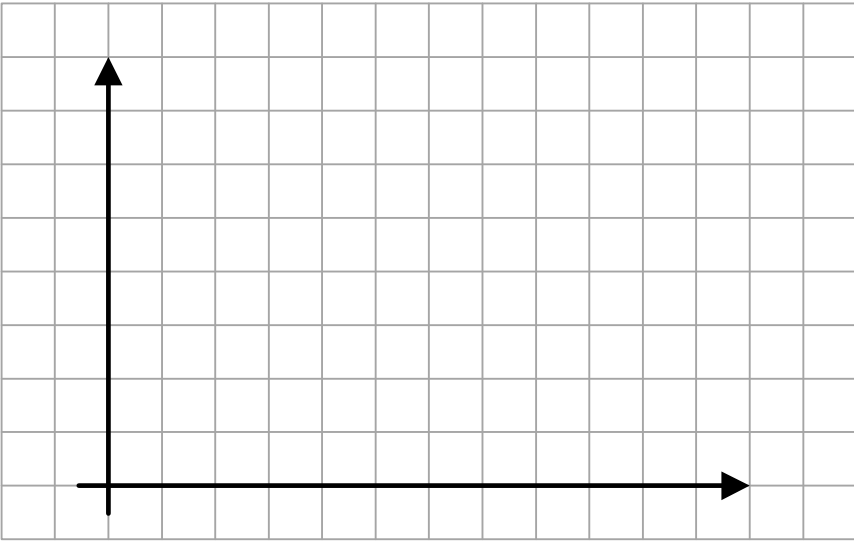
\includegraphics{normpaper.png}\\
  h) Skizzieren sie den Amplitudengang und die Sprungantwort des Filters aus f).\\
  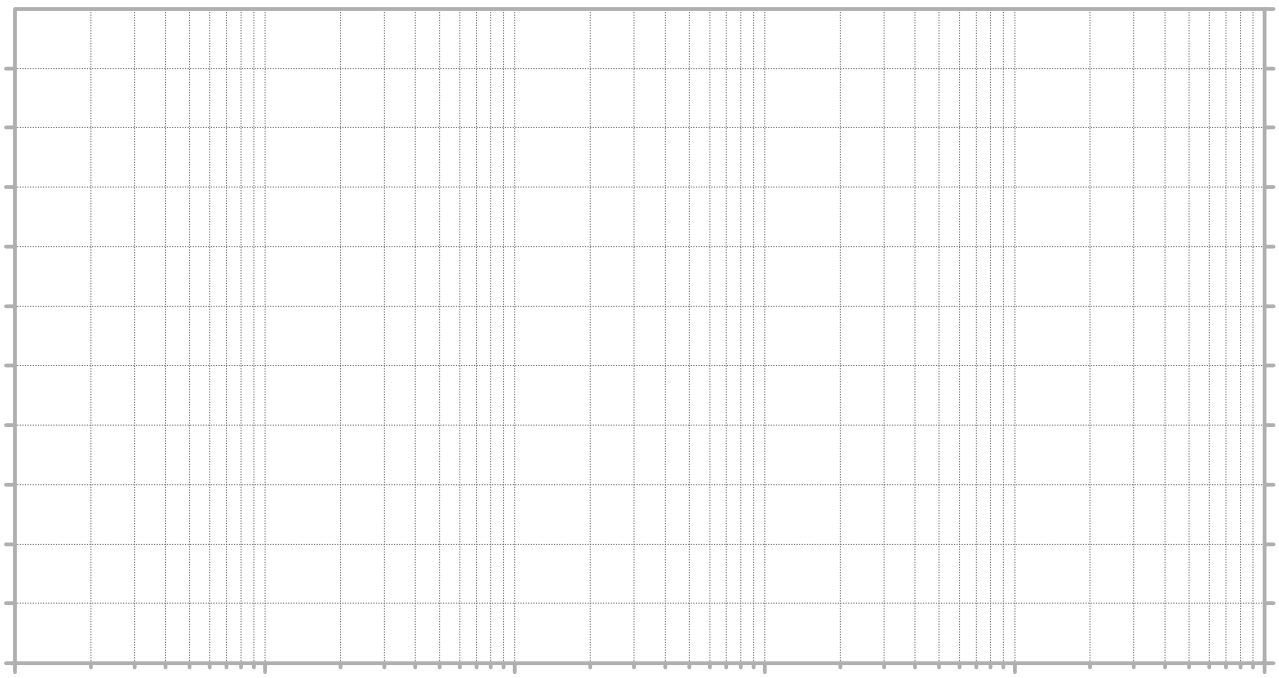
\includegraphics{logpaper.png}\\
  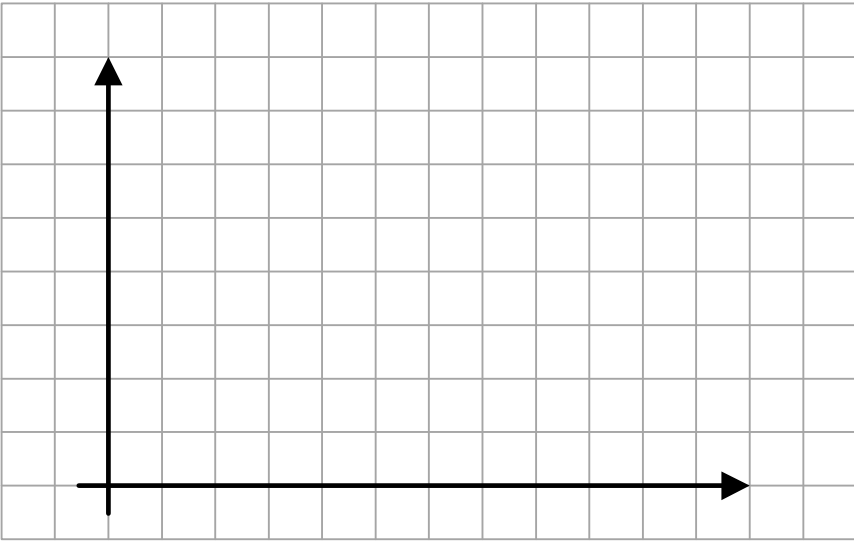
\includegraphics{normpaper.png}\\
  Zusatzfrage: Die Verstärkung des Filters soll nun auf $A_0 = 1$ verändert werden. Wie können Sie dies erreichen, ohne das Filter neu berechnen zu müssen? Zeichen sie die Schaltung mit den entsprechenden Modifikationen.

  Gegeben sei folgende Schaltung:\\
  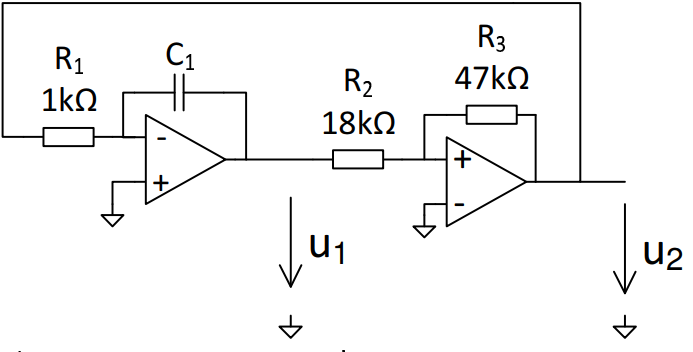
\includegraphics{Schaltung14.png}\\
  Die Aussteuergrenzen sollen mit $\pm 5V$ angenommen werden.\\
  a) Welche Ihnen bekannte Anwendungsschaltung ist hier dargestellt?\\
  b) Skizzieren sie qualitativ die Potentiale $u_1$ und $u_2$ in ein gemeinsames Diagramm.\\
  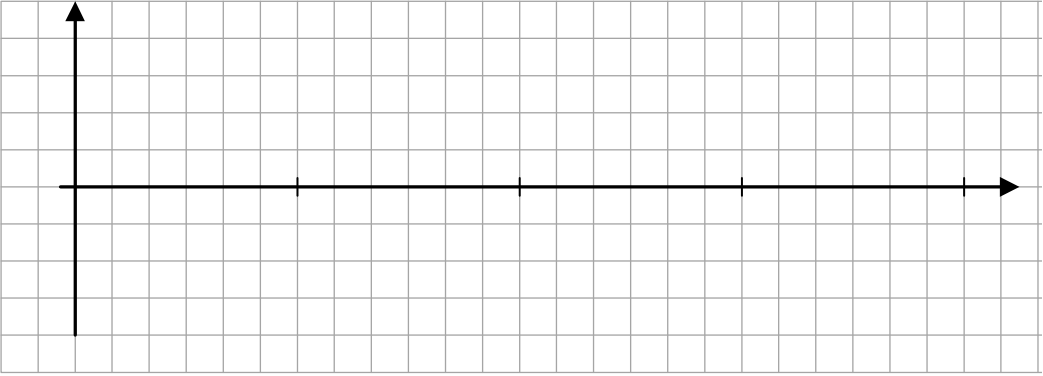
\includegraphics{pot_dia.png}\\
  c) Dimensionieren sie die Schaltung so, dass das Signal $u_1$ eine Periodendauer von $100 \mu s$ erhält. Verwenden sie Bauteile aus der E12-Reihe.\\
  d) Berechnen sie die tatsächliche Periodendauer des Signals $u_1$ für die gewählten Bauteile aus der E12-Reihe.\\
  e) Zeigen Sie, dass die Periodendauer des Ausgangssignals unabhängig von den Aussteuergrenzen des Operationsverstärkers ist?\\

  Gegeben sei folgende Schaltung:\\
  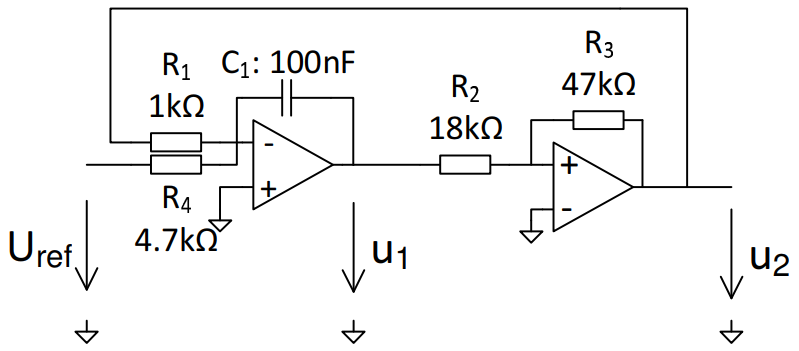
\includegraphics{Schaltung15.png}\\
  a) Stellen Sie den Zusammenhang zwischen der Spannung $U_{ref}$ und Periodendauer des Signals $u_2$ auf.\\
  Hinweis: Das resultierende Signal hat kein 50\% Tastverhältnis. Rechnen sie daher beide Fälle getrennt.\\
  b) Berechnen sie die Periodendauer und Tastverhältnis für $U_{ref} = 2.5V$.
  c) Bonusfrage: Die Schaltung wird wie folgt mit einer Diode erweitert:\\
  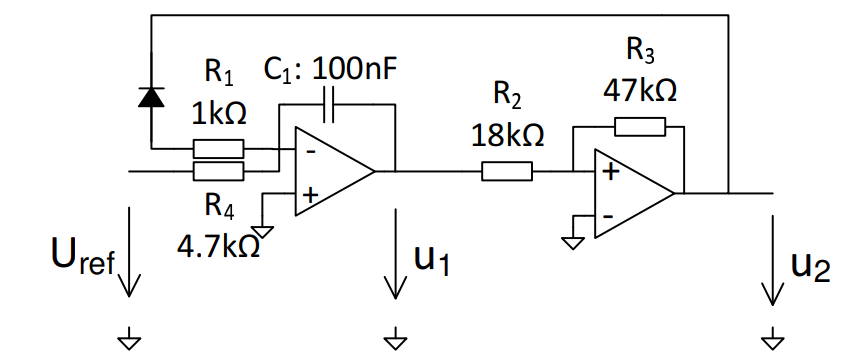
\includegraphics{Schaltung16.png}\\
  Beschreiben sie stichpunktartig den Einfluss der Diode auf die Schaltung und skizieren Sie qualitativ die Form des Signals $u_1$\\
  Hinweis: $U_{ref}$ kann für die Betrachtung als positiv und konstant angenommen werden.\\
  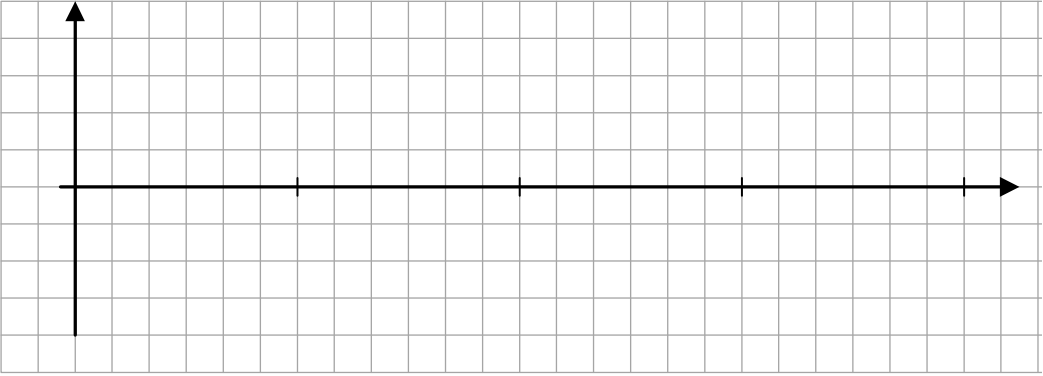
\includegraphics{pot_dia.png}

  Ein Tiefpass erster Ordnung soll entworfen werden.
  a) Zeichnen sie die Schaltung unter Verwendung eines idealen Operationsverstärkers.
  Bezeichnen sie Ein und Ausgangsspannung, sowie alle verwendeten Bauteile.\\
  b) Nennen sie die Laplace- Übertragungsfunktion der Schaltung.\\
  c) Dimensionieren Sie die Schaltung für eine Grenzfrequenz $f_c = 10Hz$, eine Eingangsimpedanz von $20k\Omega$ und einer Gleichspannungsverstärkung von $5$.\\
  Sie haben Ihrem Kommilitonen, die benötigten Bauteile gegeben und Ihn gebeten die Schaltung für sie zusammenzubauen. 
  Ihr Kommilitone kommt mit dem Ergebnis seiner "Lötkunst" zurück.
  Der Aufbau sieht auf den ersten Blick richtig aus, allerdings können Sie die passiven Bauteile aufgrund der Größe nicht unterscheiden. 
  Da Sie keine Lupe zur Hand haben, müssen Sie sich einen einfachen Test zur Funktionsüberprüfung überlegen.\\
  d) Zeichnen Sie die (drei) möglichen Schaltungen für die Permutation der Passiven Bauteile.
  e) Wie können Sie mit einem einfachen Test, die drei Varianten unterscheiden?\\
  Hinweis: sie benötigen keinen Funktionsgenerator oder Oszilloskop, eine Spannungsquelle und ein Miltimeter sind Ausreichend.\\



\end{document}
